\documentclass[12pt]{article}%
\usepackage{amsfonts}
\usepackage{fancyhdr}
\usepackage{comment}
\usepackage[a4paper, top=2.5cm, bottom=2.5cm, left=2.2cm, right=2.2cm]%
{geometry}
\usepackage{times}
\usepackage{amsmath}
\usepackage{changepage}
\usepackage{amssymb}
\usepackage{graphicx}%
\setcounter{MaxMatrixCols}{30}
\newtheorem{theorem}{Theorem}
\newtheorem{acknowledgement}[theorem]{Acknowledgement}
\newtheorem{algorithm}[theorem]{Algorithm}
\newtheorem{axiom}{Axiom}
\newtheorem{case}[theorem]{Case}
\newtheorem{claim}[theorem]{Claim}
\newtheorem{conclusion}[theorem]{Conclusion}
\newtheorem{condition}[theorem]{Condition}
\newtheorem{conjecture}[theorem]{Conjecture}
\newtheorem{corollary}[theorem]{Corollary}
\newtheorem{criterion}[theorem]{Criterion}
\newtheorem{definition}[theorem]{Definition}
\newtheorem{example}[theorem]{Example}
\newtheorem{exercise}[theorem]{Exercise}
\newtheorem{lemma}[theorem]{Lemma}
\newtheorem{notation}[theorem]{Notation}
\newtheorem{problem}[theorem]{Problem}
\newtheorem{proposition}[theorem]{Proposition}
\newtheorem{remark}[theorem]{Remark}
\newtheorem{solution}[theorem]{Solution}
\newtheorem{summary}[theorem]{Summary}
\newenvironment{proof}[1][Proof]{\textbf{#1.} }{\ \rule{0.5em}{0.5em}}

\newcommand{\Q}{\mathbb{Q}}
\newcommand{\R}{\mathbb{R}}
\newcommand{\C}{\mathbb{C}}
\newcommand{\Z}{\mathbb{Z}}

\begin{document}

\title{CS280 Fall 2018 Assignment 1 \\ Part A}
\author{ML Background}
\date{Due in class, October 12, 2018}
\maketitle

\paragraph{Name:胡志娟}

\paragraph{Student ID:67856754}

\newpage


\subsubsection*{1. MLE (5 points)}
Given a dataset $\mathcal{D} = \{x_1,\cdots, x_n\}$. Let $p_{emp}(x)$ be the empirical distribution, i.e., $p_{emp}(x)=\frac{1}{n}\sum_{i=1}^n\delta(x,x_i) $ and let $q(x|\theta)$ be some model.  
\begin{itemize}
	\item Show that $\arg\min_q KL(p_{emp}||q)$ is obtained by $q(x)=q(x;\hat{\theta})$, where $\hat{\theta}$ is the Maximum Likelihood Estimator and $KL(p||q)=\int p(x)(\log p(x)- \log q(x))dx$ is the KL divergence.
\end{itemize}

\begin{proof}\\
	Since when $n \rightarrow \infty$, the samples $q(x_i|\theta)$ will close to the empirical distribution $p_{emp}(x)$
	
	 \begin{align*}
	 &\min_q \quad KL(p_{emp}||q) \\
	 &= \min_q \quad \int p_{emp} [log(p_{emp}) - logq(x)] dx \\
	 &= \min_q \quad -\int p_{emp}logq(x)dx \\
	 &= \max_q \quad \int p_{emp}logq(x)dx \\
	 %&= \max_q \lim\limits_{n \rightarrow \infty}  \frac{1}{n} \sum_{i=1}^{n}log %q(x_i|\theta) \\
	 &= \max_q E[logq(x)] \\
	 \end{align*}
	 where Maximum Likelihood Estimator $\hat{\theta}=\arg max_q E[logq(x)] $ 
	 
	 
	 
\end{proof}





\newpage

\newpage


\subsubsection*{2. Properties of $l_2$ regularized logistic regression (10 points)}
Consider minimizing
\[
J(\mathbf{w}) = -\frac{1}{|D|}\sum_{i\in D} \log \sigma(y_i\mathbf{x}_i^T\mathbf{w})+\lambda\|\mathbf{w}\|_2^2
\]
where $y_i\in {-1,+1}$. Answer the following true/false questions and \textbf{explain why}.
\begin{itemize}
\item $J(\mathbf{w})$ has multiple locally optimal solutions: T/F?
\item Let $\hat{\mathbf{w}}=\arg\min_{\mathbf{w}}J(\mathbf{w})$ be a global optimum. $\hat{\mathbf{w}}$ is sparse (has many zeros entries): T/F?
\end{itemize}

\begin{proof}
	\begin{itemize}
		\item False. Since $J(w)$ is convex (where $-log \sigma(y_i\mathbf{x}_i^T\mathbf{w}),  \|\mathbf{w}\|_2^2$ is convex).\\
		\item False. Since $l_2$ is more smooth. From the Figure1 below, we can find that $l_2$ will prefer select more features. And for those features which are close to origin, $l_2$ norm will make them close to 0 not equal to 0 like $l_1$ norm.
		
			\begin{figure}[htbp]
				\centering
				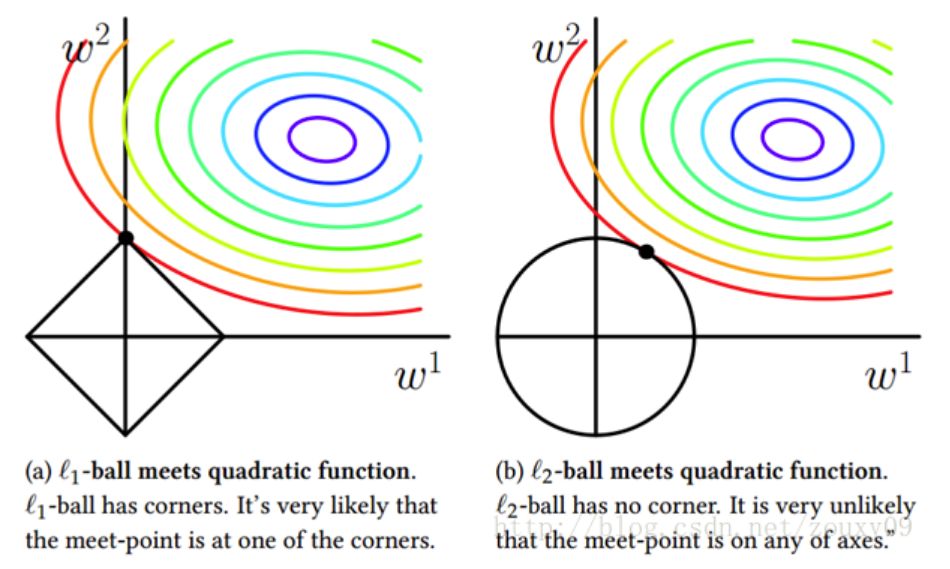
\includegraphics[width=.6\textwidth]{1.png} %1.png是图片文件的相对路径
				\caption{Comparison between $l_1$ norm and $l_2$ norm} %caption是图片的标题
				\label{img} %此处的label相当于一个图片的专属标志,目的是方便上下文的引用
			\end{figure}
		
	\end{itemize}
\end{proof}


\newpage


%\subsubsection*{3. Gaussian Distributions (10 points)}
%Let $X\sim N(0,1)$ and $Y=WX$, where $p(W=-1)=p(W=1)=0.5$. It is clear that $X$ and $Y$ are not independent since $Y$ is a function of $X$. 
%\begin{itemize}
%	\item Show $Y\sim N(0,1)$
%	\item Show $cov[X,Y]=0$. hint: $cov[X,Y]=E[XY]-E[X]E[Y]$ and $E[XY]=E[E[XY|W]]$
%\end{itemize}
%Therefore, $X$ and $Y$ are uncorrelated and Gaussian, but they are dependent. Why?
\subsubsection*{3. Gradient descent for fitting GMM (15 points)}
Consider the Gaussian mixture model
\[p(\mathbf{x}|\theta)=\sum_{k=1}^{K} \pi_{k} \mathcal{N}(\mathbf{x}|\mu_k,\Sigma_k)\]
Define the log likelihood as
\[ l(\theta) = \sum_{n=1}^N \log p(\mathbf{x}_n|\theta)
\]
Denote the posterior responsibility that cluster $k$ has for datapoint $n$ as follows:
\[
r_{nk}:=p(z_n=k|\mathbf{x}_n,\theta) = \frac{\pi_k\mathcal{N}(\mathbf{x}_n|\mu_k,\Sigma_k)}{\sum_{k'}\pi_{k'}\mathcal{N}(\mathbf{x}_n|\mu_{k'},\Sigma_k{k'})}
\]

\begin{itemize}
	
	\item Show that the gradient of the log-likelihood wrt $\mu_k$ is
	\[ \frac{d}{d\mu_k}l(\theta) = \sum_n r_{nk}\Sigma_k^{-1}(\mathbf{x}_n-\mu_k)
	\]
    \item Derive the gradient of the log-likelihood wrt $\pi_k$ without considering any constraint on $\pi_k$. (bonus: with constraint $\sum_k\pi_k=1$.)
    \item Derive the gradient of the log-likelihood wrt $\Sigma_k$ without considering any constraint on $\Sigma_k$. (bonus: with constraint $\Sigma_k$ be a symmetric positive definite matrix.) 
    
    \begin{proof}
    	
    		Suppose there are K Gauss distribution, and $x$ is a sample which obeys multi-Gauss distribution. Denoted the probability $x_i$ fall into model $k$ as:
    		$$ p(\mathbf{x_i} | z_k) =\mathcal{N}(x_i | \mu_k, \Sigma_k)$$
    		and 
    		\begin{align*}
    			p(\mathbf{x}_i|\theta) &=\sum_{k=1}^{K} \pi_{k} \mathcal{N}(\mathbf{x}|\mu_k,\Sigma_k) \\
    			&= \sum_{k=1}^{K}p(z_i=k)p(\mathbf{x}_i|z_i=k)
    		\end{align*}
    	\begin{itemize}	
    	    \item Since 
    		\begin{align*}
    		\triangledown_{\mu_k} p(\mathbf{x_n}|\theta) &= \pi_k 
    		\dfrac{1}{(2\pi)^{\frac{n}{2}} |\Sigma_k|^{\frac{1}{2}}}
    		exp\{-\frac{1}{2} (\mathbf{x_n}-\mu_k)^T\Sigma_k^{-1}(\mathbf{x_n}-\mu_k)\} \Sigma^{-1}(\mathbf{x_n}-\mu_k)  \\
    		&= \pi_k \mathcal{N}(\mathbf{x_n}| \mu_k, \Sigma_k) \Sigma_k^{-1}(\mathbf{x_n}-\mu_k)
    		\end{align*}
    		we have 
    		\begin{align*}
    			\frac{d}{d\mu_k}l(\theta) &= \sum_{n=1}^{N} \dfrac{1}{\sum_{k=1}^{K} \pi_{k} \mathcal{N}(\mathbf{x}|\mu_k,\Sigma_k)} 
    			\pi_k \mathcal{N}(\mathbf{x_n}| \mu_k, \Sigma_k) \Sigma_k^{-1}(\mathbf{x_n}-\mu_k)\\
    			&= \sum_n r_{nk}\Sigma_k^{-1}(\mathbf{x}_n-\mu_k)
    		\end{align*}
    		
    		\item Consider the MLE problem:
    		\begin{align*}
    			&\max l(\theta) \\
    			&s.t. \sum_{k=1}^{K} \pi_k=1
    		\end{align*}
    		Using Lagrange Multiplier method, construct Lagrange function:
    		\begin{align*}
    		\mathcal{L}(\pi_k) = l(\theta) + \lambda(1-\sum_{k=1}^{K}\pi_k) 
    		\end{align*}
    		Since 
    		\begin{align}
    		\dfrac{p(\mathbf{x}_n|\theta)}{d\pi_k} &= \mathcal{N}(\mathbf{x}_n|\mu_k, \Sigma_k) \\
    		\dfrac{\mathcal{L}(\pi_k)}{d\pi_k} &= \dfrac{d}{d\pi_k}l(\theta) - \lambda =0 
    		\end{align}
    		we have
    		\begin{align*}
    		\dfrac{d}{d\pi_k}l(\theta) 
    		&= \dfrac{d}{d\pi_k} \sum_{i=1}^{n} logp(\mathbf{x}_n|\theta) \\
    		&= \sum_{i=1}^{n} \frac{1}{p(\mathbf{x}_n|\theta)} \frac{d p(\mathbf{x}_n|\theta)}{d\pi_k} \\
    		&= \sum_{i=1}^{n} \frac{1}{p(\mathbf{x}_n|\theta)} \mathcal{N}(\mathbf{x}_n|\mu_k, \Sigma_k) \\
    		&= \sum_{i=1}^{n} \dfrac{r_{nk}}{\pi_k}
    		\end{align*}
    		Using (2) and $\sum_{k=1}^{K}\pi_k=1$, we have
    		\begin{align*}
    		\lambda &=\sum_{i=1}^{n} \dfrac{r_{nk}}{\pi_k} \\
    		&= N
    		\end{align*}
    		
    		
    		\item From the equation
    		\begin{align}
    			\dfrac{\partial log(f(x))}{\partial x} &= \frac{1}{f(x)} \frac{\partial f(x)}{\partial x} \\
    			\Rightarrow \quad \dfrac{\partial f(x)}{\partial x} &= f(x)\dfrac{\partial log(f(x))}{\partial x}
    		\end{align}
    		
    		Using (4), we have
    		%\begin{align}
    		%\dfrac{d}{d\Sigma_k}p(\mathbf{\mathbf{x}_i|\theta)} &=
    		%\dfrac{d}{d\Sigma_k} \sum_{i=1}^{k} p(z_k) p(\mathbf{x}_i|z_k) \\
    		%&= \sum_{i=1}^{k}p(z_k)p(\mathbf{x}_i|z_k) \dfrac{d log}{d %\Sigma_k}[\sum_{i=1}^{k}p(z_k)p(\mathbf{x}_i|z_k)] \\
    		%&= \sum_{i=1}^{k}p(z_k)p(\mathbf{x}_i|z_k) %\dfrac{dlog}{d\Sigma_k}p(z_k)p(\mathbf{x}_i|z_k) \\
    		%&= \sum_{i=1}^{k}p(z_k)p(\mathbf{x}_i|z_k)
            %\dfrac{dlog}{d\Sigma_k}p(\mathbf{x}_i|\mu_k,\Sigma_k)
    		%\end{align}
    		
    		\begin{align}
    		\dfrac{d}{d\Sigma_k}p(\mathbf{\mathbf{x}_i|\theta)} &=
    		\dfrac{d}{d\Sigma_k} \sum_{i=1}^{k} p(z_k) p(\mathbf{x}_i|z_k)\\
    		&= \dfrac{d}{d\Sigma_k} p(z_k) p(\mathbf{x}_i|z_k) \\
    		&= p(z_k) \dfrac{d}{d\Sigma_k} p(\mathbf{x}_i|z_k) \\
    		&= p(z_k) p(\mathbf{x}_i|z_k) \dfrac{dlog}{d\Sigma_k}p(\mathbf{x}_i|\mu_k,\Sigma_k)
    		\end{align}
    		
    		Since \begin{align}
    		tr(ABC) &= tr(CAB) \\
    		\dfrac{dtr(BA)}{dA} &=B^T\\
    		\dfrac{dtr(A^{-1}B)}{dA} &=-(A^{-1})^TB(A^{-1})^T
    		\end{align}
    		
    		For \begin{align}
    		\dfrac{dlog}{d\Sigma_k}p(\mathbf{x}_i|\mu_k,\Sigma_k) 
    		&=\dfrac{dlog}{d\Sigma_k} \left[ \dfrac{1}{(2\pi)^{\frac{n}{2}} |\Sigma_k|^{\frac{1}{2}}}
    		exp\{-\frac{1}{2} (\mathbf{x_n}-\mu_k)^T\Sigma_k^{-1}(\mathbf{x_n}-\mu_k)\} \Sigma^{-1}(\mathbf{x_n}-\mu_k) \right] \\
    		&= \dfrac{d}{d\Sigma_k} \left[-\frac{1}{2}log(|\Sigma_k|) -\frac{1}{2} (\mathbf{x_n}-\mu_k)^T\Sigma_k^{-1}(\mathbf{x_n}-\mu_k)\} \Sigma^{-1}(\mathbf{x_n}-\mu_k)
    		\right] \\
    		&= (-\frac{1}{2}) \left[ \Sigma_k^{-1} - \Sigma_k^{-1}(\mathbf{x}_i - \mu_k)(\mathbf{x}_i - \mu_k)^T\Sigma_k^{-1} \right]
    		\end{align}
    		
    		Hence, combine (8) and (14), equation (5) has
    		\begin{align}
    		\dfrac{d}{d\Sigma_k}p(\mathbf{\mathbf{x}_i|\theta)} 
    		&= p(z_k)p(\mathbf{x}_i|z_k)
    		(-\frac{1}{2}) \left[ \Sigma_k^{-1} - \Sigma_k^{-1}(\mathbf{x}_i - \mu_k)(\mathbf{x}_i - \mu_k)^T\Sigma_k^{-1} \right]\\
    		&= \pi_k\mathcal{N}(\mathbf{x}_i|\mu_k,\Sigma_k) 
    		(-\frac{1}{2}) \left[ \Sigma_k^{-1} - \Sigma_k^{-1}(\mathbf{x}_i - \mu_k)(\mathbf{x}_i - \mu_k)^T\Sigma_k^{-1} \right]
    		\end{align}
    		
    		At last, since
    		\begin{align}
    		\dfrac{d}{d\Sigma_k} l(\theta) &= \dfrac{d}{d\Sigma_k} \sum_{i=1}^{N}log p(\mathbf{x_i}|\theta) \\
    		&=  \dfrac{1}{p(\mathbf{x}|\theta)}  \dfrac{d}{d\Sigma_k} p(\mathbf{x}_k|\theta) \\
    		&=  \dfrac{\pi_k\mathcal{N}(\mathbf{x}_i|\mu_k,\Sigma_k)}
    		{\sum_{i=1}^{k}\pi_k\mathcal{N}(\mathbf{x}_i|\mu_k,\Sigma_k)}
    		(-\frac{1}{2}) \left[ \Sigma_k^{-1} - \Sigma_k^{-1}(\mathbf{x}_i - \mu_k)(\mathbf{x}_i - \mu_k)^T\Sigma_k^{-1} \right]
    		\end{align}
    		
    		 
    	\end{itemize}
    	
    	
    	
    	
    \end{proof}
    
	
\end{itemize}


\end{document}\grid
\grid
\grid
